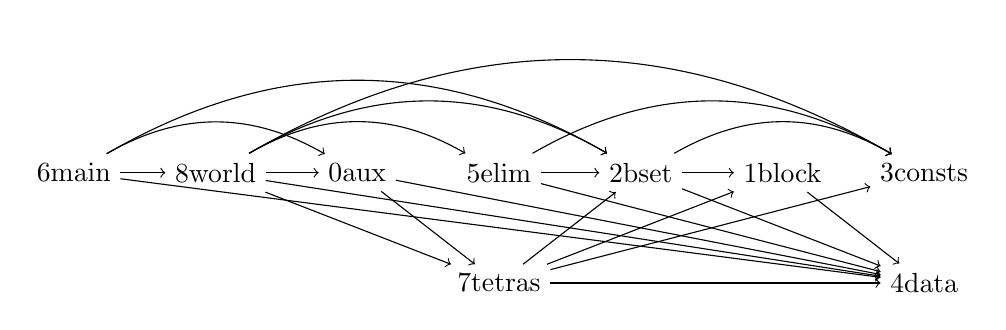
\begin{tikzpicture}

  \node (00)  {\rkt{3}{consts}};
  \node (01) [below of=00,yshift=-0.4cm] {\rkt{4}{data}};
  \node (10) [left of=00,xshift=-0.8cm] {\rkt{1}{block}};
  \node (20) [left of=10,xshift=-0.8cm] {\rkt{2}{bset}};
  \node (30) [left of=20,xshift=-0.8cm] {\rkt{5}{elim}};
  \node (31) [below of=30,yshift=-0.4cm] {\rkt{7}{tetras}};
  \node (40) [left of=30,xshift=-0.8cm] {\rkt{0}{aux}};
  \node (50) [left of=40,xshift=-0.8cm] {\rkt{8}{world}};
  \node (60) [left of=50,xshift=-0.8cm] {\rkt{6}{main}};

  \draw[->] (10) -- (01);
  \draw[->] (20) edge[bend left] (00);
  \draw[->] (20) -- (10);
  \draw[->] (20) -- (01);
  \draw[->] (30) edge[bend left] (00);
  \draw[->] (30) -- (20);
  \draw[->] (30) -- (01);
  \draw[->] (31) -- (10);
  \draw[->] (31) -- (00);
  \draw[->] (31) -- (01);
  \draw[->] (31) -- (20);
  \draw[->] (40) -- (31);
  \draw[->] (40) -- (01);
  \draw[->] (50) edge[bend left] (00);
  \draw[->] (50) edge[bend left] (30);
  \draw[->] (50) -- (40);
  \draw[->] (50) -- (31);
  \draw[->] (50) edge[bend left] (20);
  \draw[->] (50) -- (01);
  \draw[->] (60) -- (01);
  \draw[->] (60) edge[bend left] (20);
  \draw[->] (60) -- (50);
  \draw[->] (60) edge[bend left] (40);

\end{tikzpicture}
